%%%%%%%%%%%%%%%%%%%%%%%%%%%%%%%%%%%%%%%%%
% Beamer Presentation
% LaTeX Template
% Version 1.0 (10/11/12)
%
% This template has been downloaded from:
% http://www.LaTeXTemplates.com
%
% License:
% CC BY-NC-SA 3.0 (http://creativecommons.org/licenses/by-nc-sa/3.0/)
%
%%%%%%%%%%%%%%%%%%%%%%%%%%%%%%%%%%%%%%%%%

%----------------------------------------------------------------------------------------
%	PACKAGES AND THEMES
%----------------------------------------------------------------------------------------

%\documentclass[UTF8,aspectratio=169,14pt]{ctexbeamer}
\documentclass[UTF8,aspectratio=169]{ctexbeamer}
\usepackage{hyperref}
\hypersetup{
	colorlinks=true,
	linkcolor=red,
	anchorcolor=blue,
	citecolor=green
}

\mode<presentation> {
	
	% The Beamer class comes with a number of default slide themes
	% which change the colors and layouts of slides. Below this is a list
	% of all the themes, uncomment each in turn to see what they look like.
	
	%\usetheme{default}
	%\usetheme{AnnArbor}
	%\usetheme{Antibes}
	%\usetheme{Bergen}
	%\usetheme{Berkeley}
	%\usetheme{Berlin}
	%\usetheme{Boadilla}
	%\usetheme{CambridgeUS}
	%\usetheme{Copenhagen}
	%\usetheme{Darmstadt}
	%\usetheme{Dresden}
	%\usetheme{Frankfurt}
	%\usetheme{Goettingen}
	%\usetheme{Hannover}
	%\usetheme{Ilmenau}
	%\usetheme{JuanLesPins}
	%\usetheme{Luebeck}
	\usetheme{Madrid}
	%\usetheme{Malmoe}
	%\usetheme{Marburg}
	%\usetheme{Montpellier}
	%\usetheme{PaloAlto}
	%\usetheme{Pittsburgh}
	%\usetheme{Rochester}
	%\usetheme{Singapore}
	%\usetheme{Szeged}
	%\usetheme{Warsaw}
	
	% As well as themes, the Beamer class has a number of color themes
	% for any slide theme. Uncomment each of these in turn to see how it
	% changes the colors of your current slide theme.
	
	%\usecolortheme{albatross}
	%\usecolortheme{beaver}
	%\usecolortheme{beetle}
	%\usecolortheme{crane}
	%\usecolortheme{dolphin}
	%\usecolortheme{dove}
	%\usecolortheme{fly}
	%\usecolortheme{lily}
	%\usecolortheme{orchid}
	%\usecolortheme{rose}
	%\usecolortheme{seagull}
	%\usecolortheme{seahorse}
	%\usecolortheme{whale}
	%\usecolortheme{wolverine}
	
	%\setbeamertemplate{footline} % To remove the footer line in all slides uncomment this line
	%\setbeamertemplate{footline}[page number] % To replace the footer line in all slides with a simple slide count uncomment this line
	
	%\setbeamertemplate{navigation symbols}{} % To remove the navigation symbols from the bottom of all slides uncomment this line
}

\usepackage{graphicx} % Allows including images
\graphicspath{{./figs/}}
\usepackage{booktabs} % Allows the use of \toprule, \midrule and \bottomrule in tables
\usepackage{longtable}
\usepackage{listings}
\usepackage{xcolor}
\lstset{numbers=left, %设置行号位置
	numberstyle=\tiny, %设置行号大小
	keywordstyle=\color{blue}, %设置关键字颜色
	commentstyle=\color[cmyk]{1,0,1,0}, %设置注释颜色
	frame=single, %设置边框格式
	escapeinside=``, %逃逸字符(1左面的键),用于显示中文
	%breaklines, %自动折行
	extendedchars=false, %解决代码跨页时,章节标题,页眉等汉字不显示的问题
	xleftmargin=2em,xrightmargin=2em, aboveskip=1em, %设置边距
	tabsize=4, %设置tab空格数
	showspaces=false %不显示空格
}
% Fonts
% \usepackage{libertine}
% \setmonofont{Courier}
\setCJKsansfont[ItalicFont=Noto Serif CJK SC Black, BoldFont=Noto Sans CJK SC Black]{Noto Sans CJK SC}
\setmainfont[Ligatures={Common,TeX}]{Linux  Libertine O}
\setmonofont[SmallCapsFont={Latin Modern Mono Caps}]{Latin Modern Mono Light}
\setsansfont{Linux Biolinum O}

\logo{
\includegraphics[width=0.55cm,height=0.55cm]{../../thcs-logo.png}}

%----------------------------------------------------------------------------------------
%	TITLE PAGE
%----------------------------------------------------------------------------------------

\title[第5讲]{第5讲 :The Interface of OS} % The short title appears at the bottom of every slide, the full title is only on the title page
\subtitle{第四节:How to design a Linux kernel interface}
\author{陈渝} % Your name
\institute[清华大学] % Your institution as it will appear on the bottom of every slide, may be shorthand to save space
{
	清华大学计算机系 \\ % Your institution for the title page
	\medskip
	\textit{yuchen@tsinghua.edu.cn} % Your email address
}
\date{\today} % Date, can be changed to a custom date


\begin{document}

\begin{frame}
\titlepage % Print the title page as the first slide
\end{frame}

%\begin{frame}
%\frametitle{提纲} % Table of contents slide, comment this block out to remove it
%\tableofcontents % Throughout your presentation, if you choose to use \section{} and \subsection{} commands, these will automatically be printed on this slide as an overview of your presentation
%\end{frame}
%
%%----------------------------------------------------------------------------------------
%%	PRESENTATION SLIDES
%%----------------------------------------------------------------------------------------
%
%%------------------------------------------------
%\section{第一节:课程概述} % Sections can be created in order to organize your presentation into discrete blocks, all sections and subsections are automatically printed in the table of contents as an overview of the talk
%%------------------------------------------------
%-------------------------------------------------
\begin{frame}[plain]
	\frametitle{Introduction}
	
	
	

			\centering
			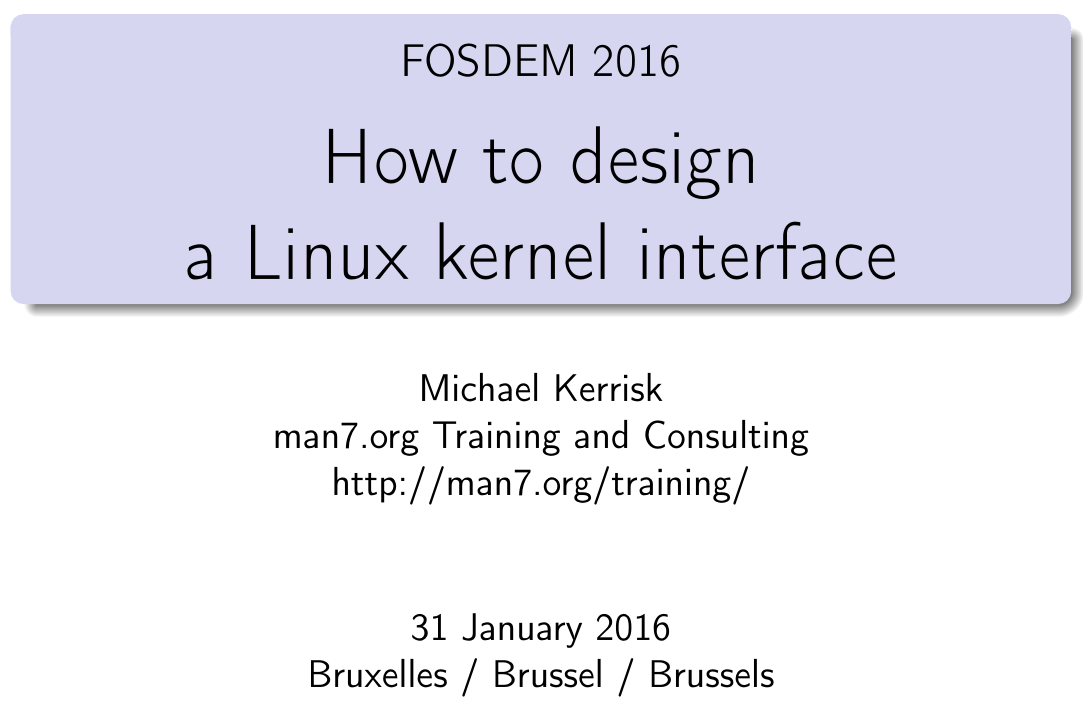
\includegraphics[width=.5\textwidth]{howto-design-linux-kernel-interface}
			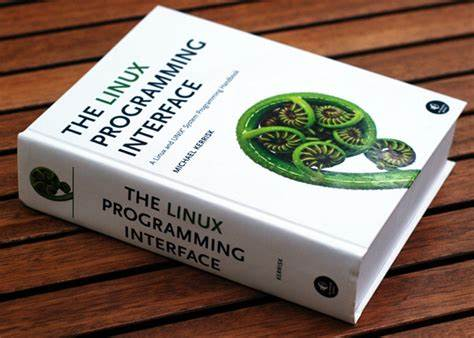
\includegraphics[width=.4\textwidth]{book-tlpi}

	
\end{frame}



%-------------------------------------------------
\begin{frame}[plain]
	\frametitle{Introduction}
	
	
	
	\begin{columns}
		
		\begin{column}{.4\textwidth}
			
			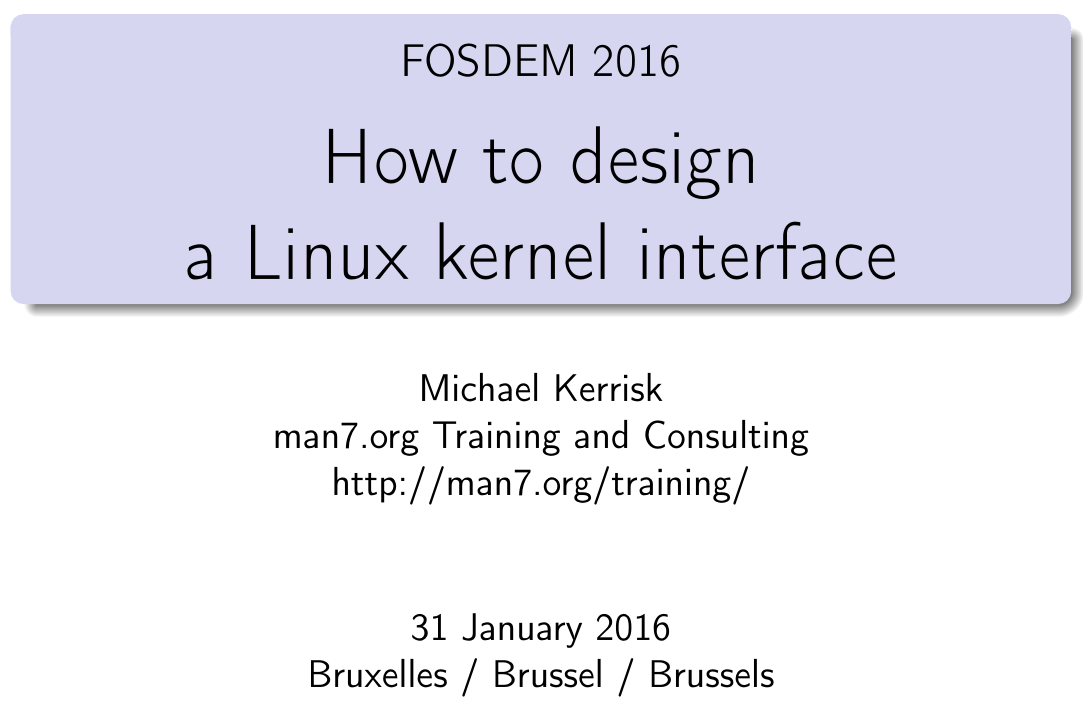
\includegraphics[width=1.\textwidth]{howto-design-linux-kernel-interface}
			
		\end{column}
		
		\begin{column}{.6\textwidth}
			\LARGE
			\begin{block}{Moral 1: diverse user usages}
				try to imagine the ways
				in which an army of inventive
				user-space programmers might
				(ab)use your API
				
			\end{block} 
		\normalsize
		3.5 MQ changes also
		broke user space
		in at least two places
		\begin{itemize}
			\item Introduced hard limit of 1024 on queues\_max, Fixed by commit f3713fd9c
			\item Semantics of value exported in /dev/mqueue QSIZE field
			changed
			
		\end{itemize}
		\end{column}
		
		
	\end{columns}
	
	
\end{frame}



%-------------------------------------------------
\begin{frame}[plain]
	\frametitle{Introduction}
	
	
	
	\begin{columns}
		
		\begin{column}{.4\textwidth}
			
			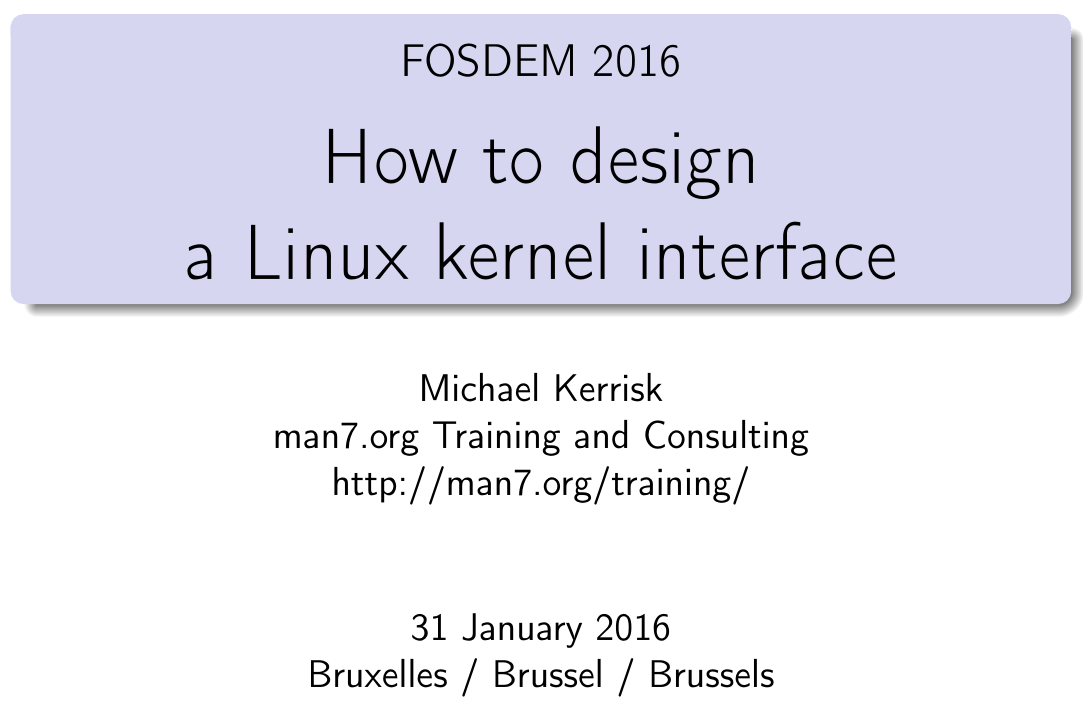
\includegraphics[width=1.\textwidth]{howto-design-linux-kernel-interface}
			
		\end{column}
		
		\begin{column}{.6\textwidth}
			\LARGE
			\begin{block}{Moral 2 : unit tests}
				without unit tests you
				will screw up someone’s API
			\end{block} 
			\normalsize
			Regressions happen more often
			than you’d expect
			
			\begin{itemize}
				\item Linux 2.6.12 silently changed meaning of fcntl() F\_SETOWN				
				\item No longer possible to target signals at specific thread in
				multithreaded process
			
			\end{itemize}
		
			Inotify IN\_ONESHOT flag
		
			\begin{itemize}
			\item By design, IN\_ONESHOT did not cause an IN\_IGNORED event
			when watch is dropped after one event
							
			\item From 2.6.36, IN\_ONESHOT does cause IN\_IGNORED
			
				
			\end{itemize}

		\end{column}
		
		
	\end{columns}
	
	
\end{frame}


%-------------------------------------------------
\begin{frame}[plain]
	\frametitle{Introduction}
	
	
	
	\begin{columns}
		
		\begin{column}{.4\textwidth}
			
			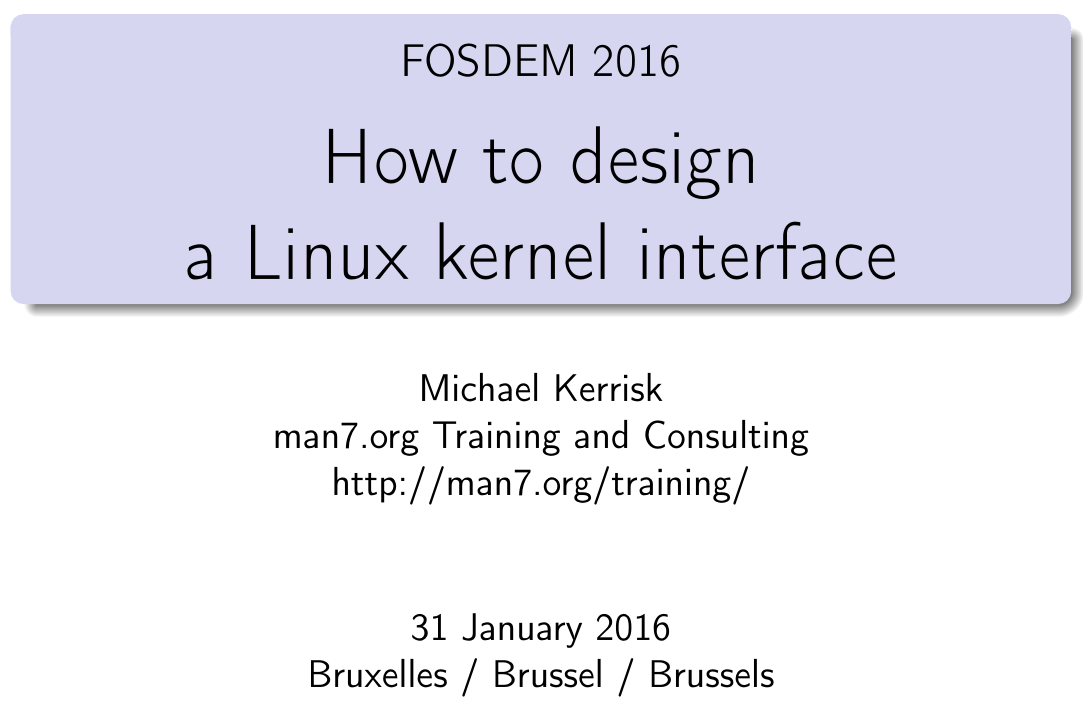
\includegraphics[width=1.\textwidth]{howto-design-linux-kernel-interface}
			
		\end{column}
		
		\begin{column}{.6\textwidth}
			\Large
			\begin{block}{Moral 3: Specification, Andrew Morton}
				Programming is not just an act of telling a computer
				what to do: it is also an act of telling other
				programmers what you wished the computer to do.
				Both are important, and the latter deserves care. 
				
				
			\end{block} 
			\normalsize
			recvmmsg() timeout argument needed a specification; something like:
			
			\begin{itemize}
				\item timeout is NULL
				\item timeout points to {0, 0}
				\item timeout points to a structure which is nonzero. 
				\item If, while blocking, the call is interrupted by a signal handler,
%				,then
%				if 1 or more datagrams have been received, then those datagrams
%				are returned (and interruption by a signal handler is not (directly)
%				reported by this or any subsequent call to recvmmsg().
%				if no datagrams have so far been received, then the call fails with
%				the error EINTR.
%				Man pages as a test specification

				Specification, Andrew Morton
			\end{itemize}
		\end{column}
		
		
	\end{columns}
	
	
\end{frame}



%-------------------------------------------------
\begin{frame}[plain]
	\frametitle{Introduction}
	
	
	
	\begin{columns}
		
		\begin{column}{.4\textwidth}
			
			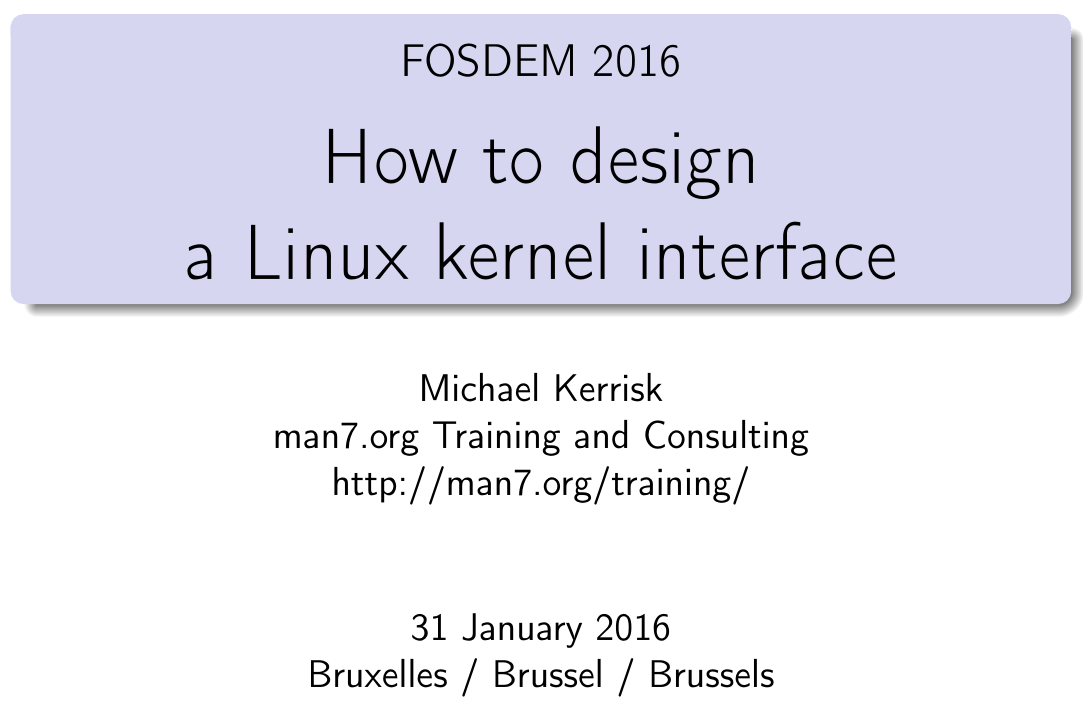
\includegraphics[width=1.\textwidth]{howto-design-linux-kernel-interface}
			
		\end{column}
		
		\begin{column}{.6\textwidth}
			\Large
			\begin{block}{Moral 4: feedback loop}
				Strive to shorten worst-case
				feedback loop. Publicize API design
				as widely + early as possible.		
					
			\end{block} 
		
			\normalsize
			Ideally, do all of the following before API release:
			
			\begin{itemize}
				\item Write a detailed specification
				\item Write example programs that fully demonstrate API				
				\item Email relevant mailing lists and, especially, relevant people, CC linux-api@vger.kernel.org
				
				\item write an LWN.net article
				
			\end{itemize}
		\end{column}
		
		
	\end{columns}
	
	
\end{frame}


%-------------------------------------------------
\begin{frame}[plain]
	\frametitle{Introduction}
	
	
	
	\begin{columns}
		
		\begin{column}{.4\textwidth}
			
			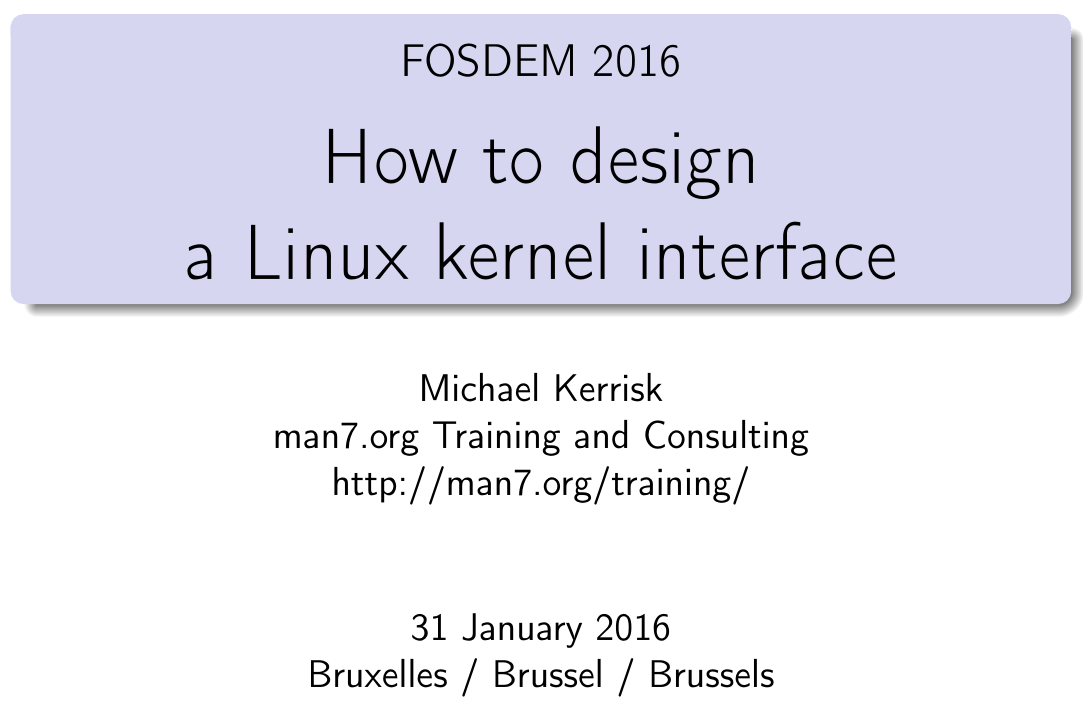
\includegraphics[width=1.\textwidth]{howto-design-linux-kernel-interface}
			
		\end{column}
		
		\begin{column}{.6\textwidth}
			\Large
			\begin{block}{Moral 5: into real world}
				Only way to discover design
				problems in a new nontrivial API
				is by writing complete, real-world
				application(s)	
				
			\end{block} 
			
			\normalsize
			Writing a “real” inotify application
			
			
			\begin{itemize}
				\item Back story: I thought I understood inotify
				
				\item Then I tried to write a “real” application(500 lines of C with (lots of) comments)...
						
				\item Written up on LWN (https://lwn.net/Articles/605128/)
				
				
				\item And understood all the work that inotify still leaves you to do
				
				
			\end{itemize}
		\end{column}
		
		
	\end{columns}
	
	
\end{frame}



%-------------------------------------------------
\begin{frame}[plain]
	\frametitle{Introduction}
	
	
	
	\begin{columns}
		
		\begin{column}{.4\textwidth}
			
			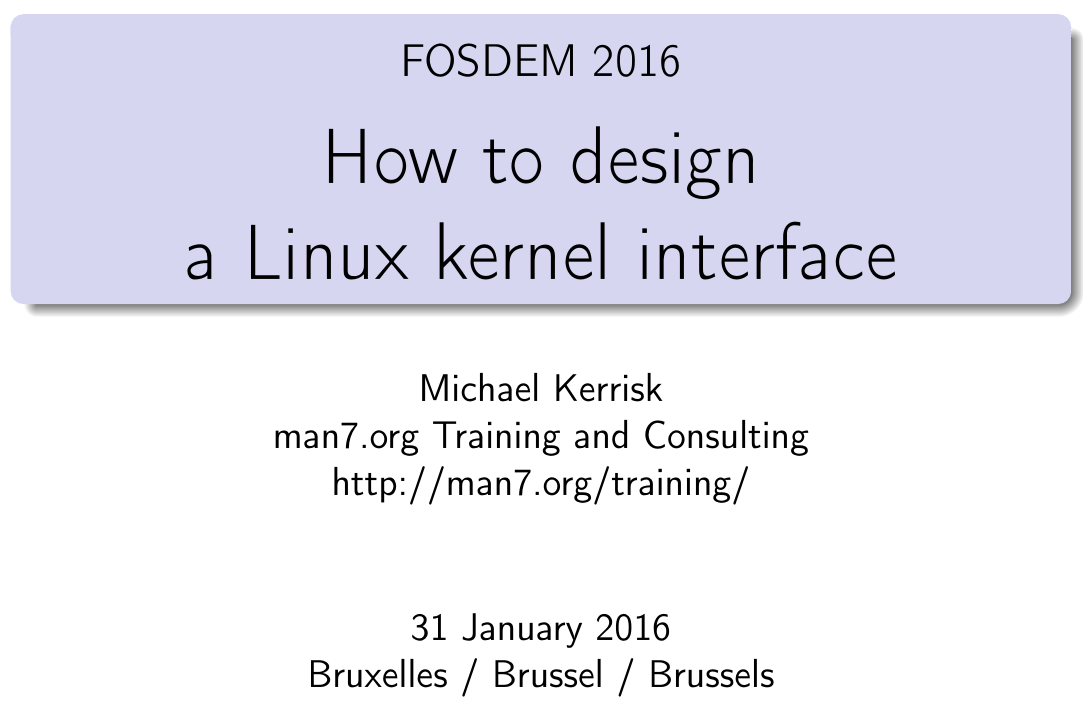
\includegraphics[width=1.\textwidth]{howto-design-linux-kernel-interface}
			
		\end{column}
		
		\begin{column}{.6\textwidth}
			\large
			\begin{block}{Moral 6: technical checklist	}
			\begin{itemize}
			\item New system calls should allow for extensibility. 

			\item Undefined arguments and flags must be zero. 
			\item Syscalls with timeouts should allow absolute timeouts 
			\item Avoid extending multiplexor system calls
			\item etc.
		    \end{itemize}
			\end{block} 
			
			

		\end{column}
		
		
	\end{columns}
	
	
\end{frame}
%-------------------------------------------------

%-------------------------------------------------
\end{document}